\chapter{Projektauftrag}
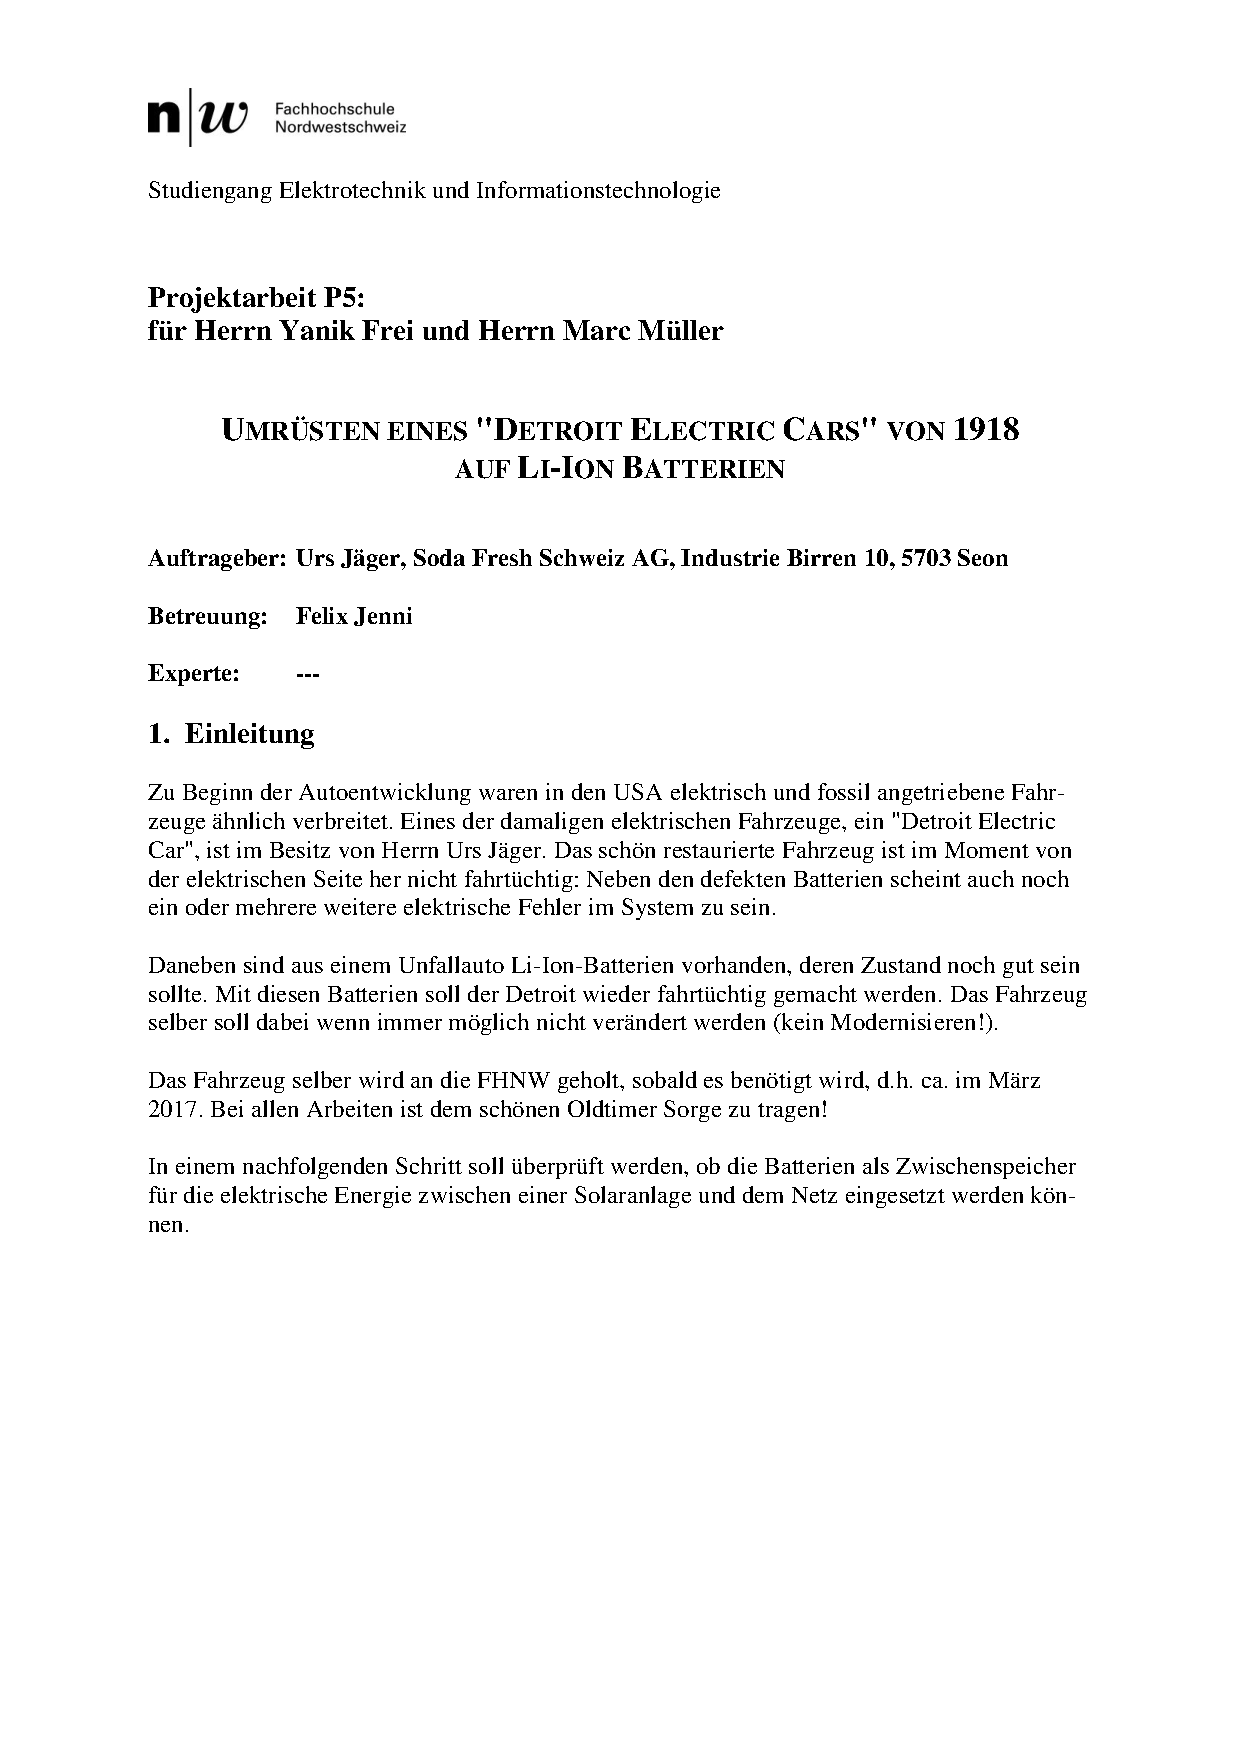
\includepdf[pages=-]{P5_Frei_Mueller.pdf}
%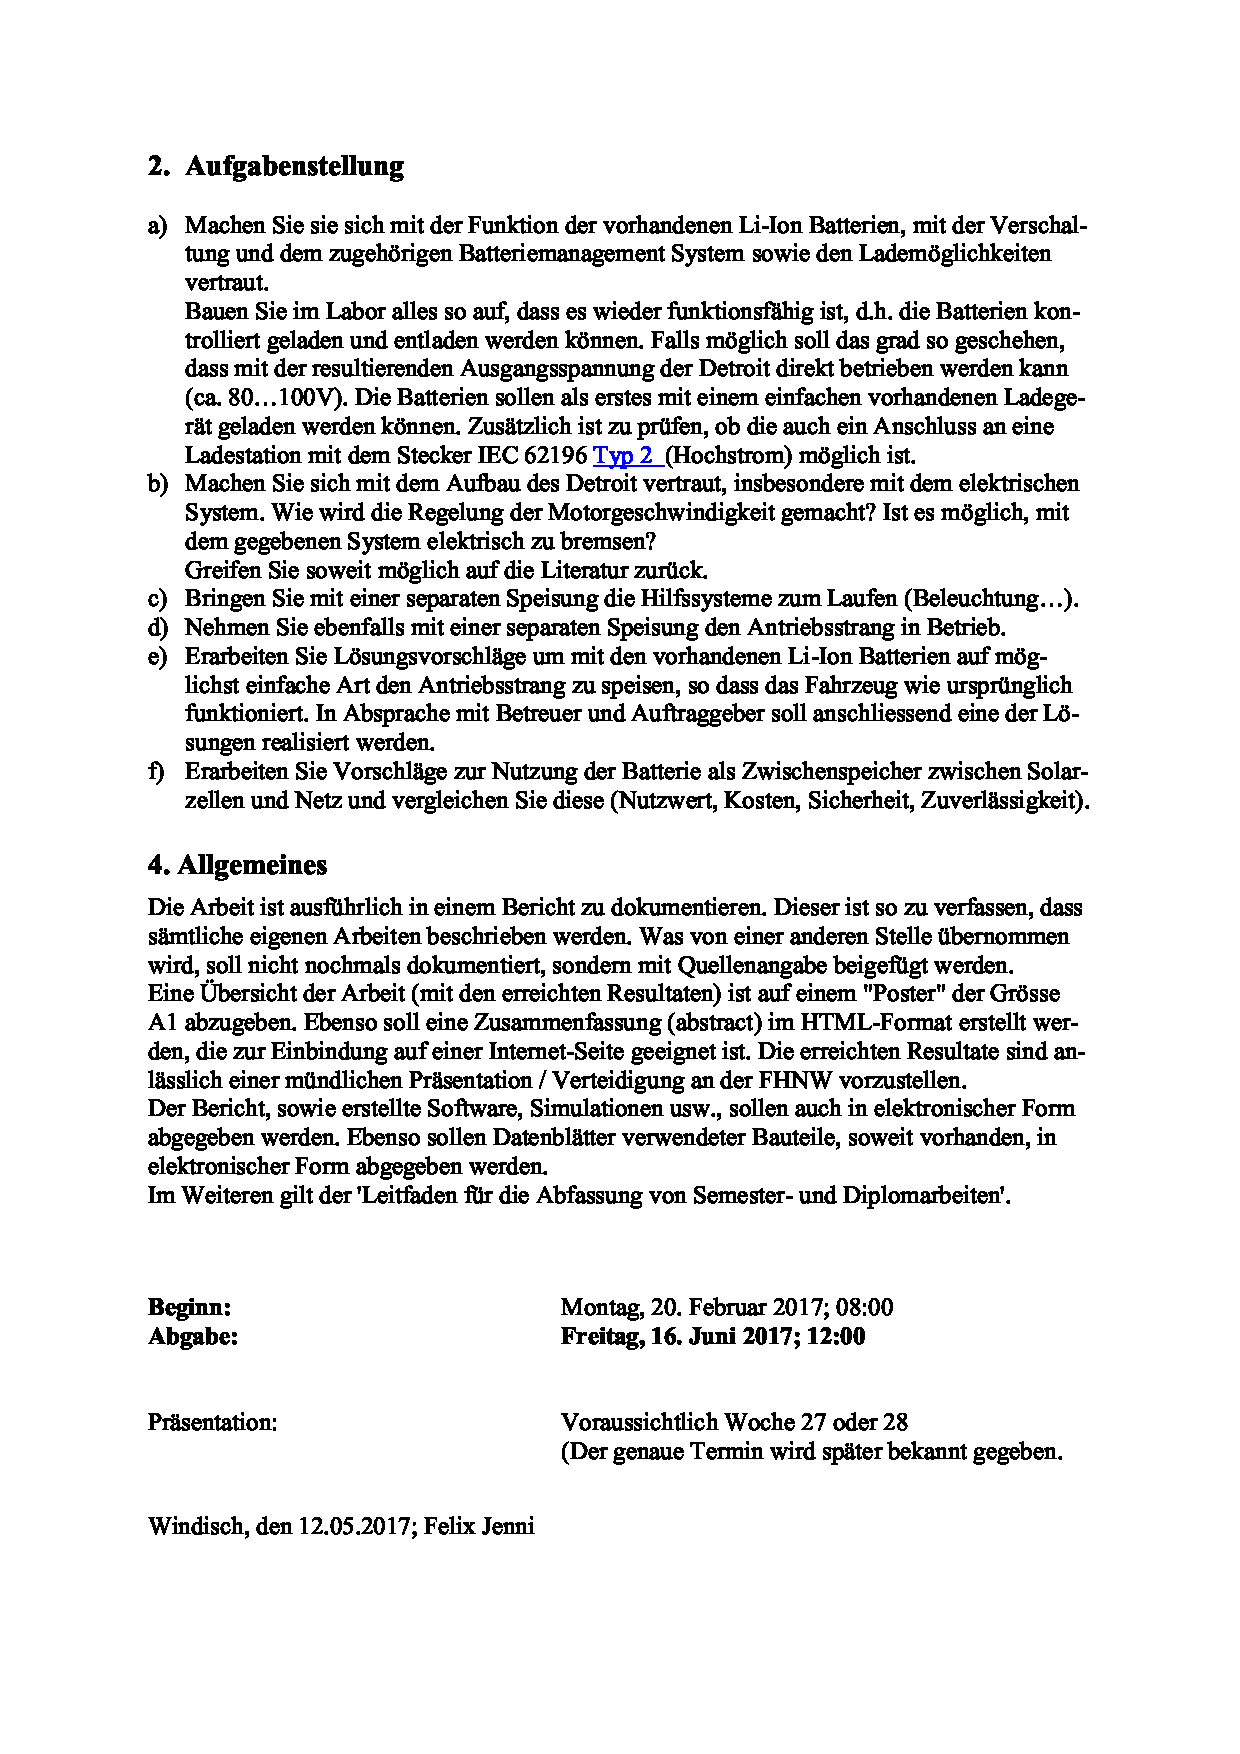
\includepdf{P5_Frei_Mueller2.pdf}
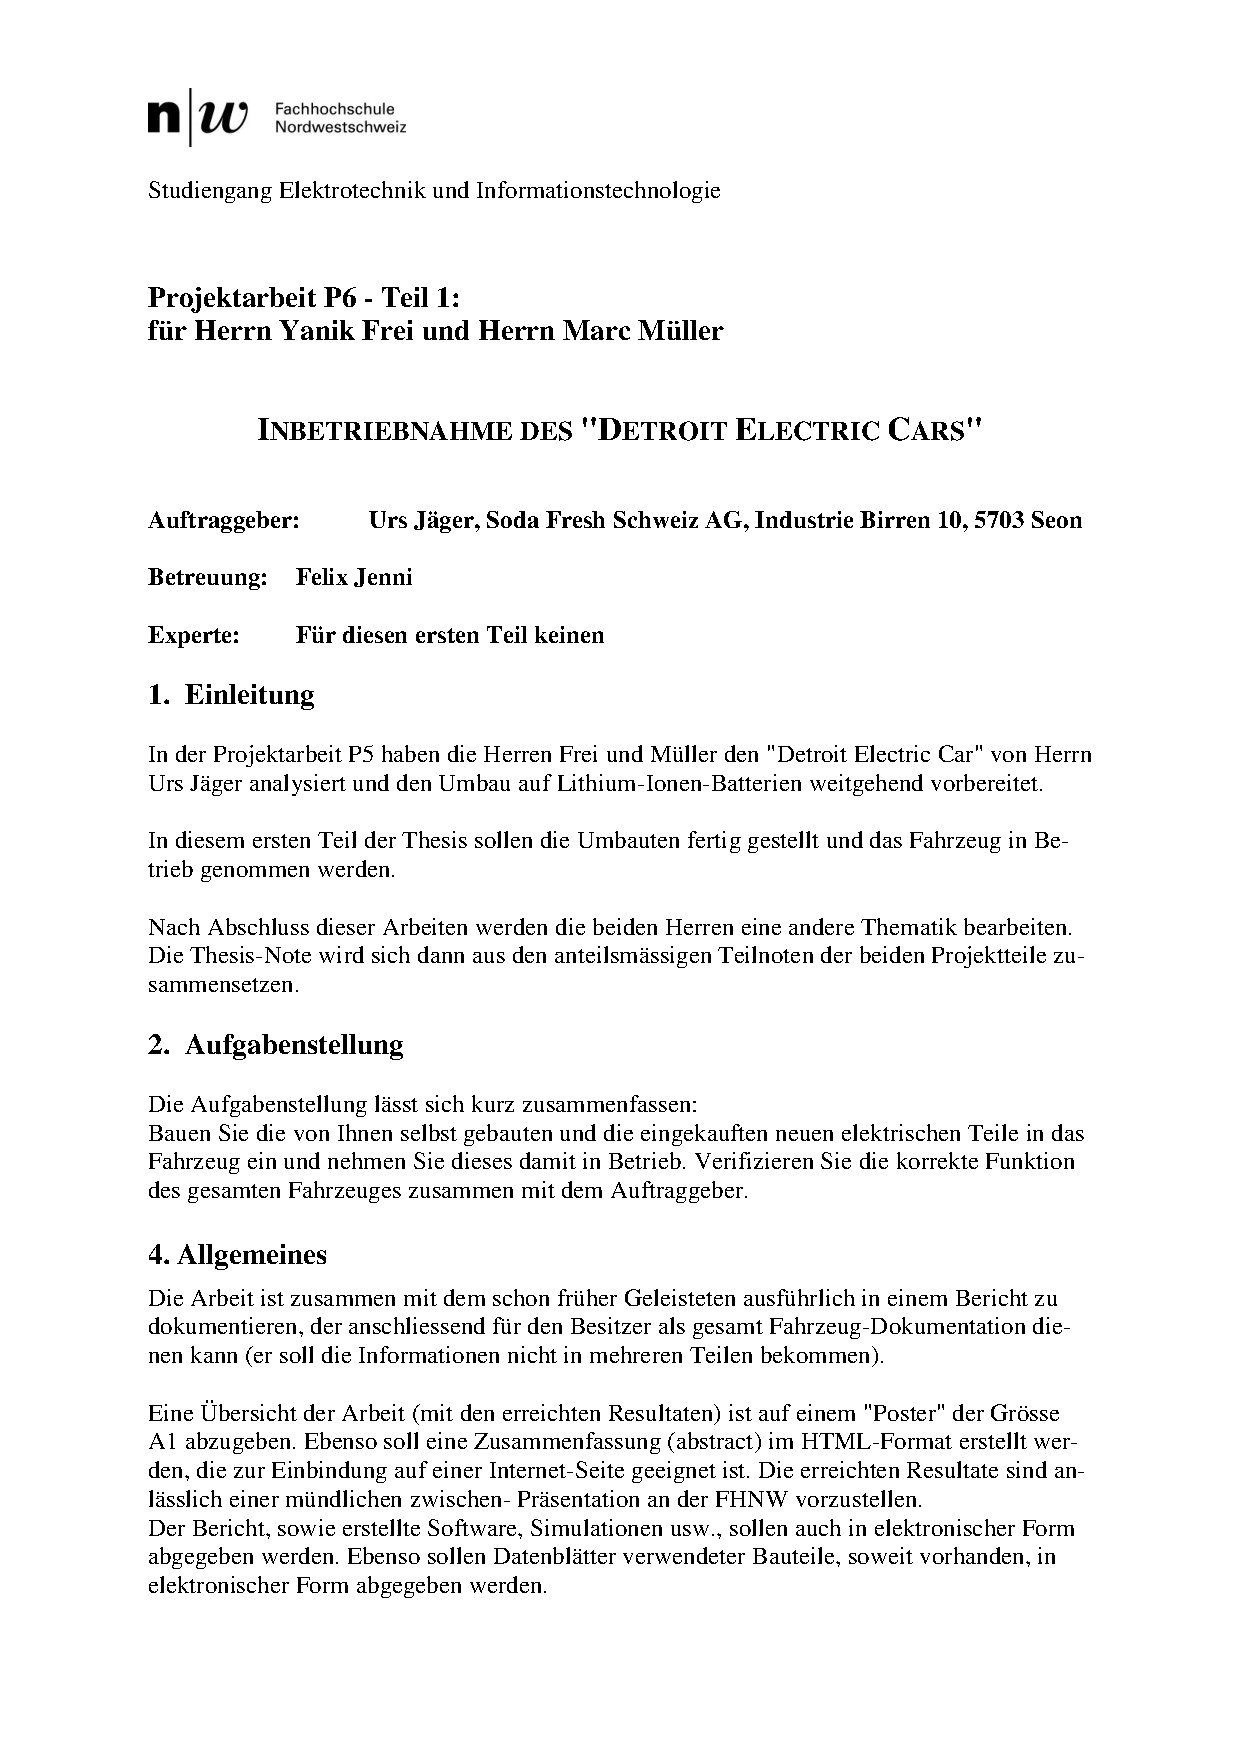
\includepdf[pages=-]{P6_Teil_1_Frei_Mueller.pdf}
%
\includepdf{P6_Teil_1_Frei_Mueller2.pdf}

\chapter{Original Starkstromschema}\label{schema_original}
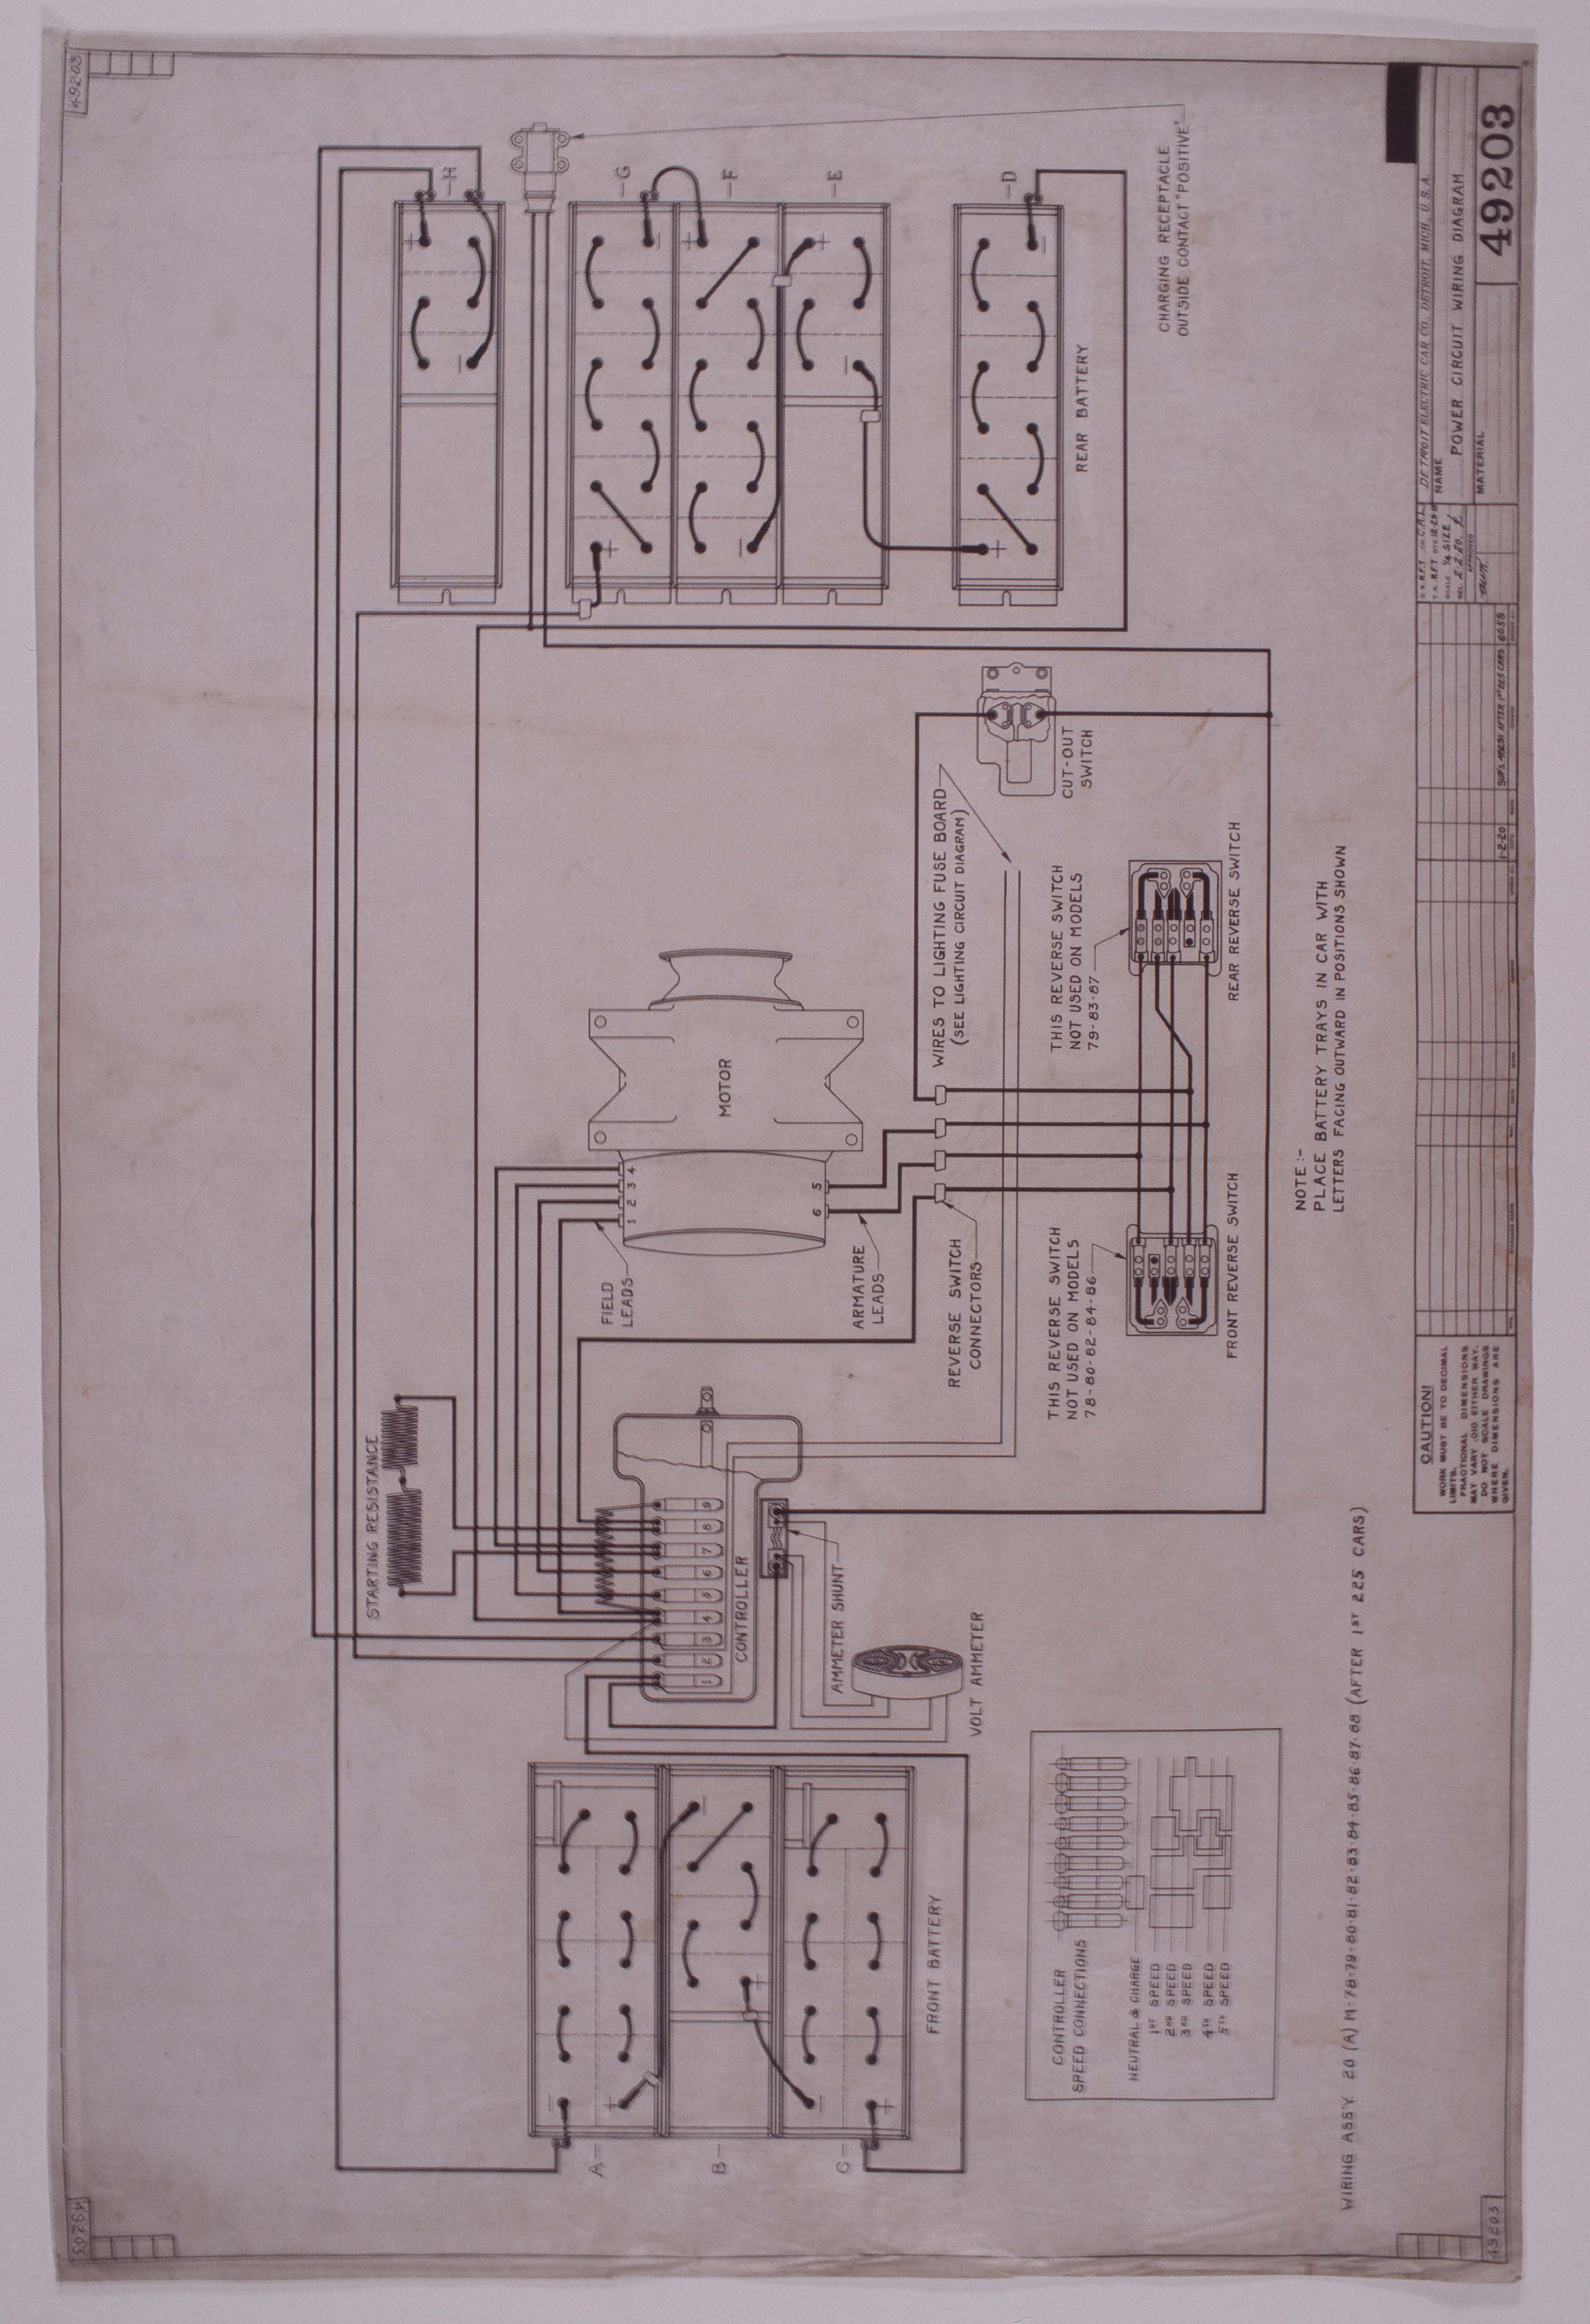
\includepdf{images/Schema_Starkstrom_Detroit.pdf}

\chapter{Original Lichtschema}\label{app:licht}
\includepdf{images/Schema_Licht_Detroit.pdf}

\chapter{Schema Steuerplatine}\label{Anh_Steuerplatine}
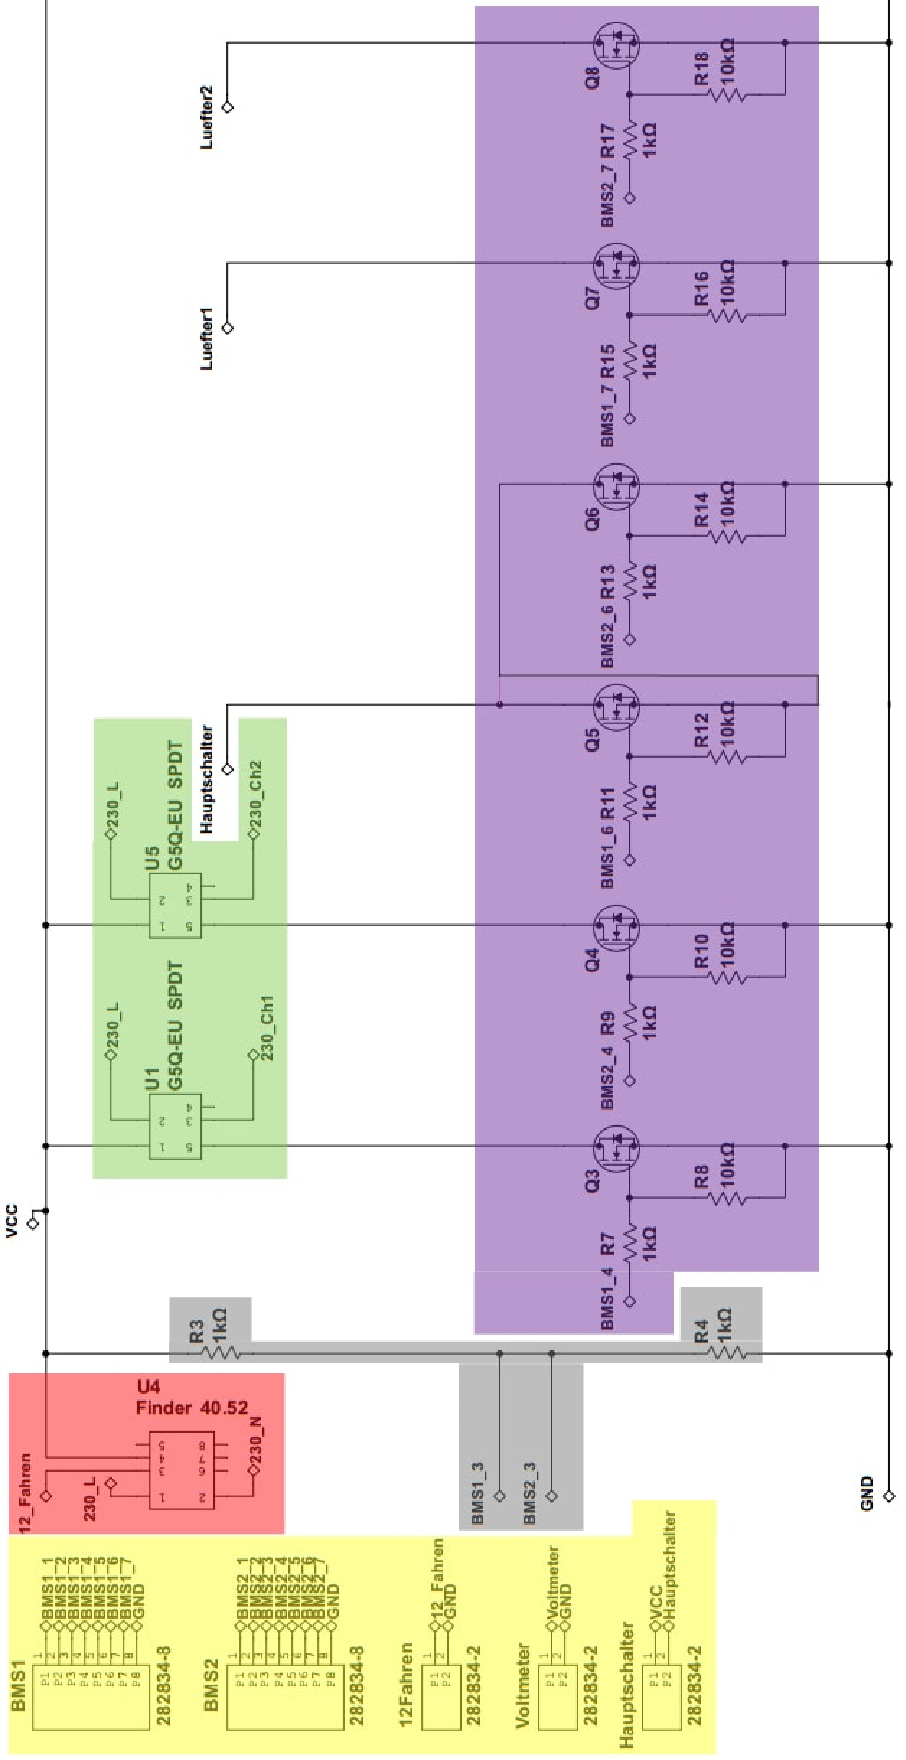
\includepdf{images/Steuerplatine_1.pdf}
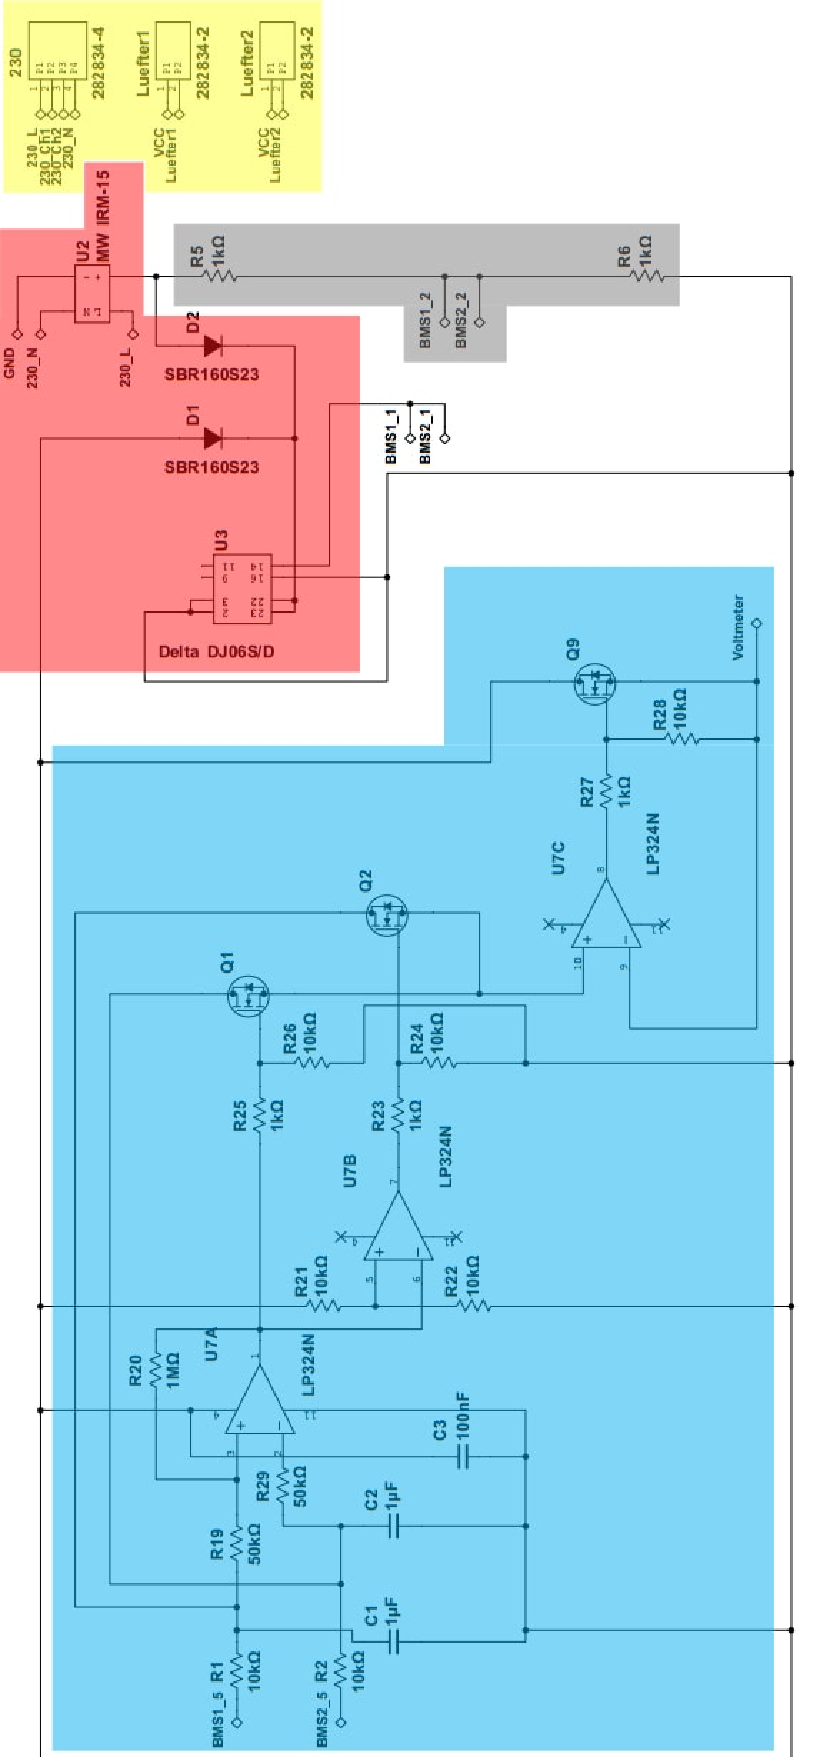
\includepdf{images/Steuerplatine_2.pdf}

\chapter{Zeichnungen neuer Shunt}\label{app:2d}
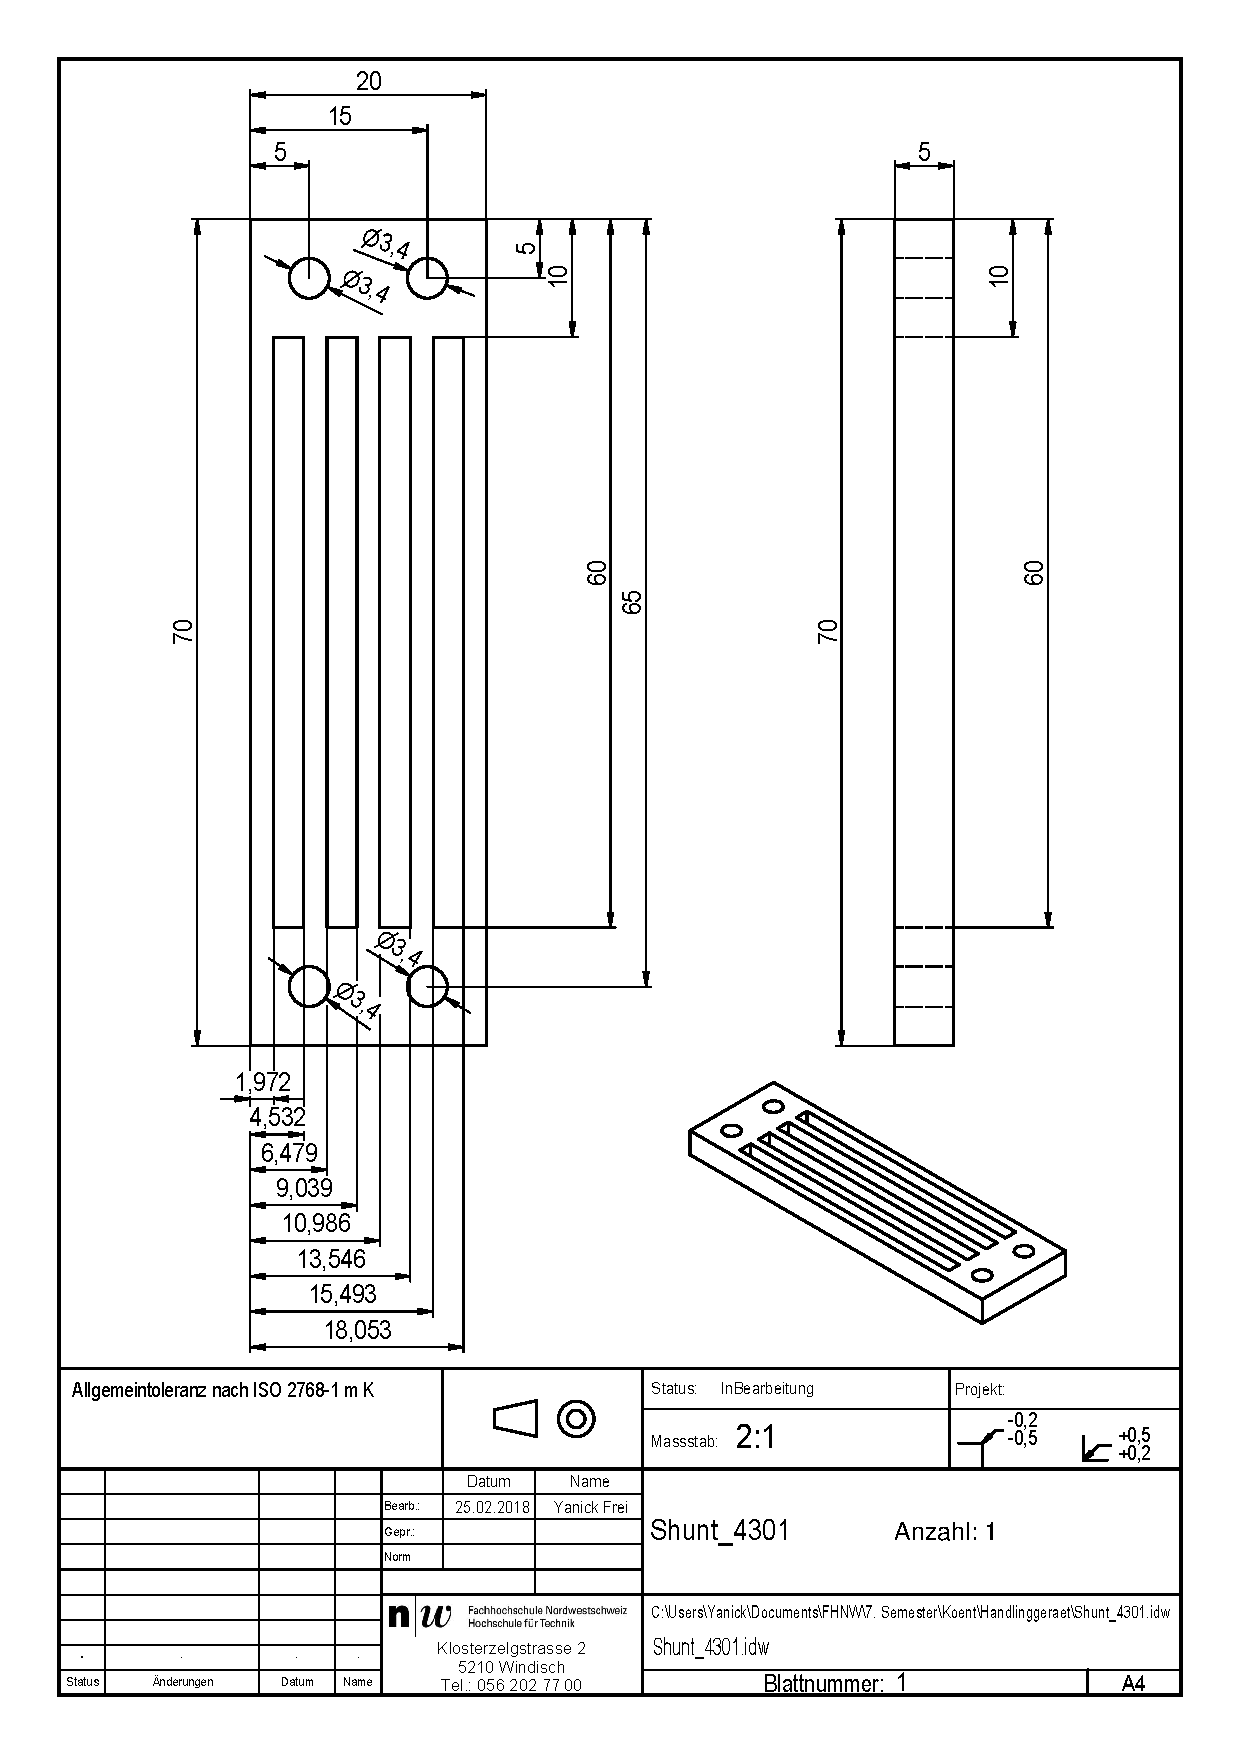
\includepdf{images/Shunt_4301.pdf}
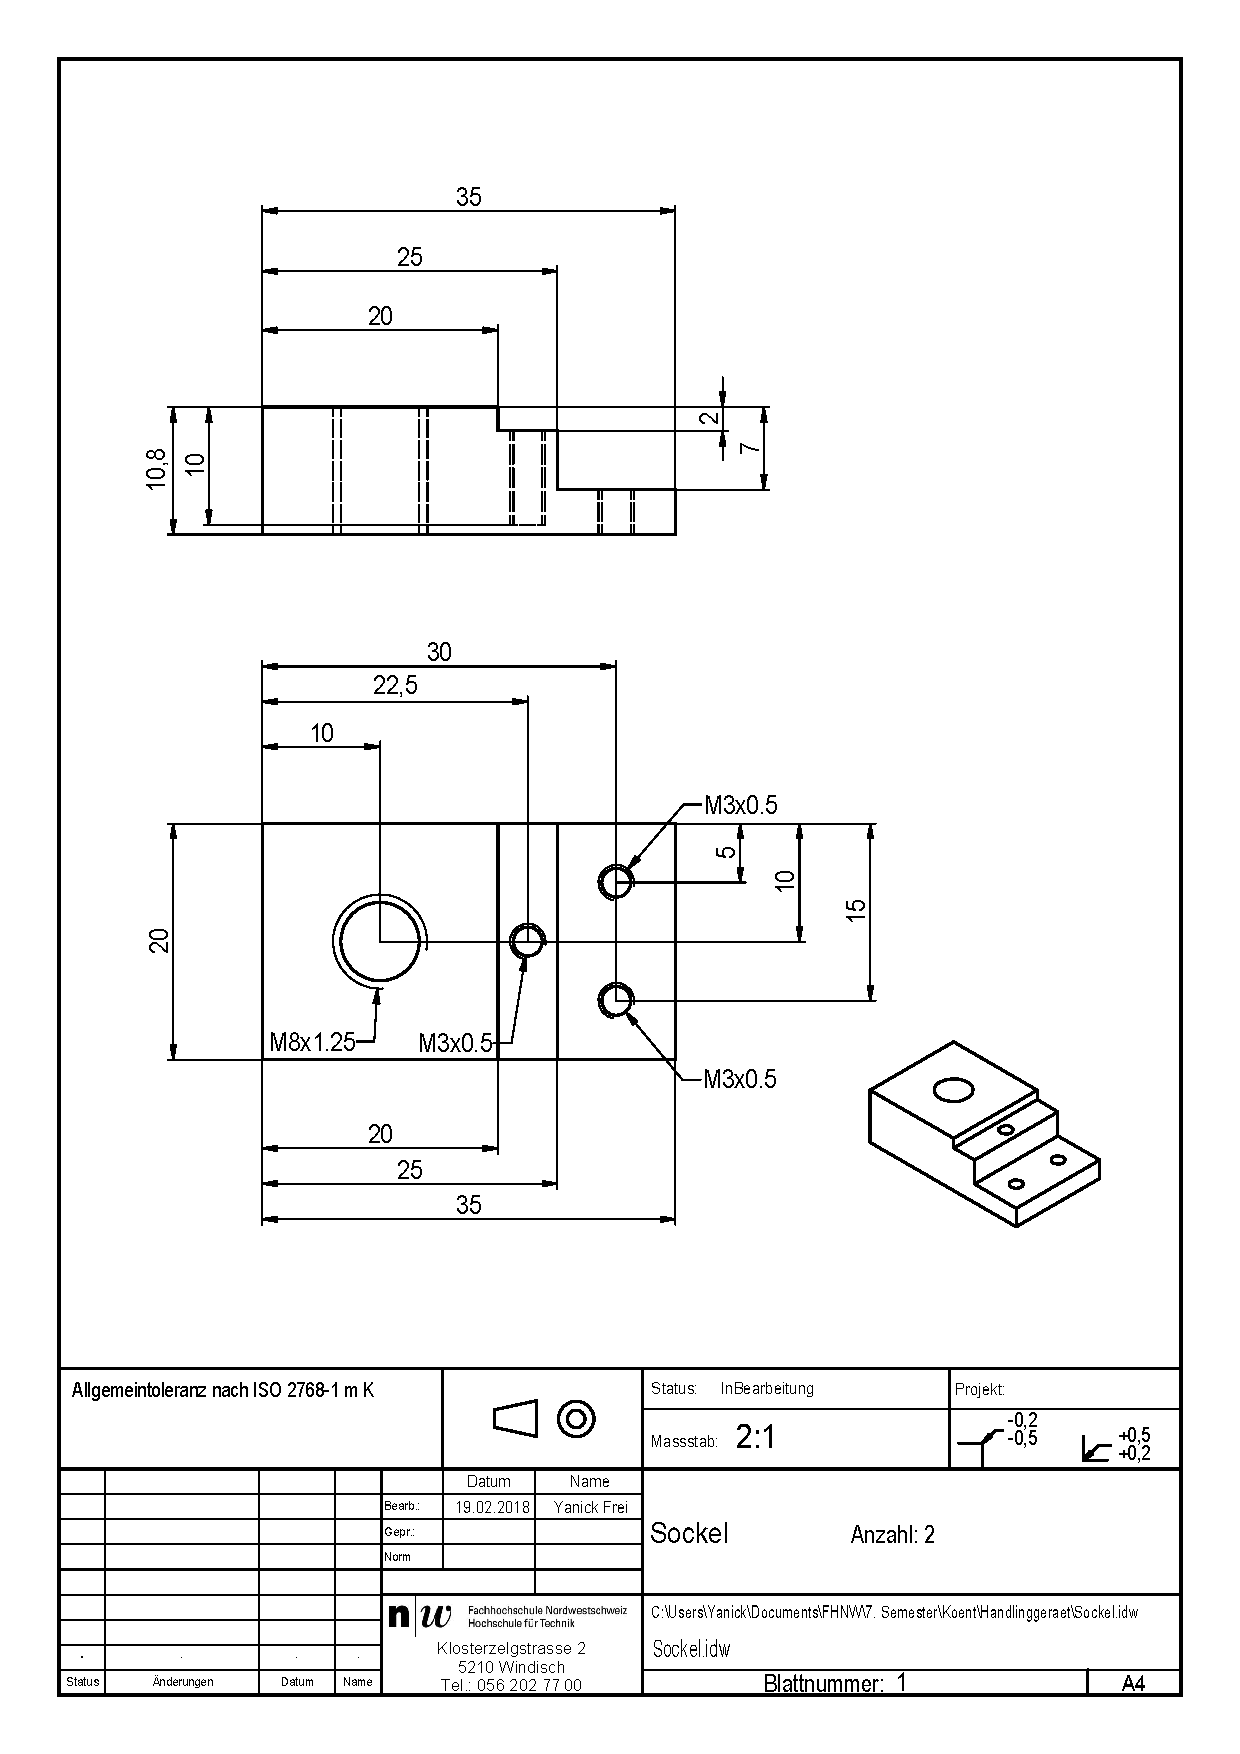
\includepdf{images/Sockel.pdf}
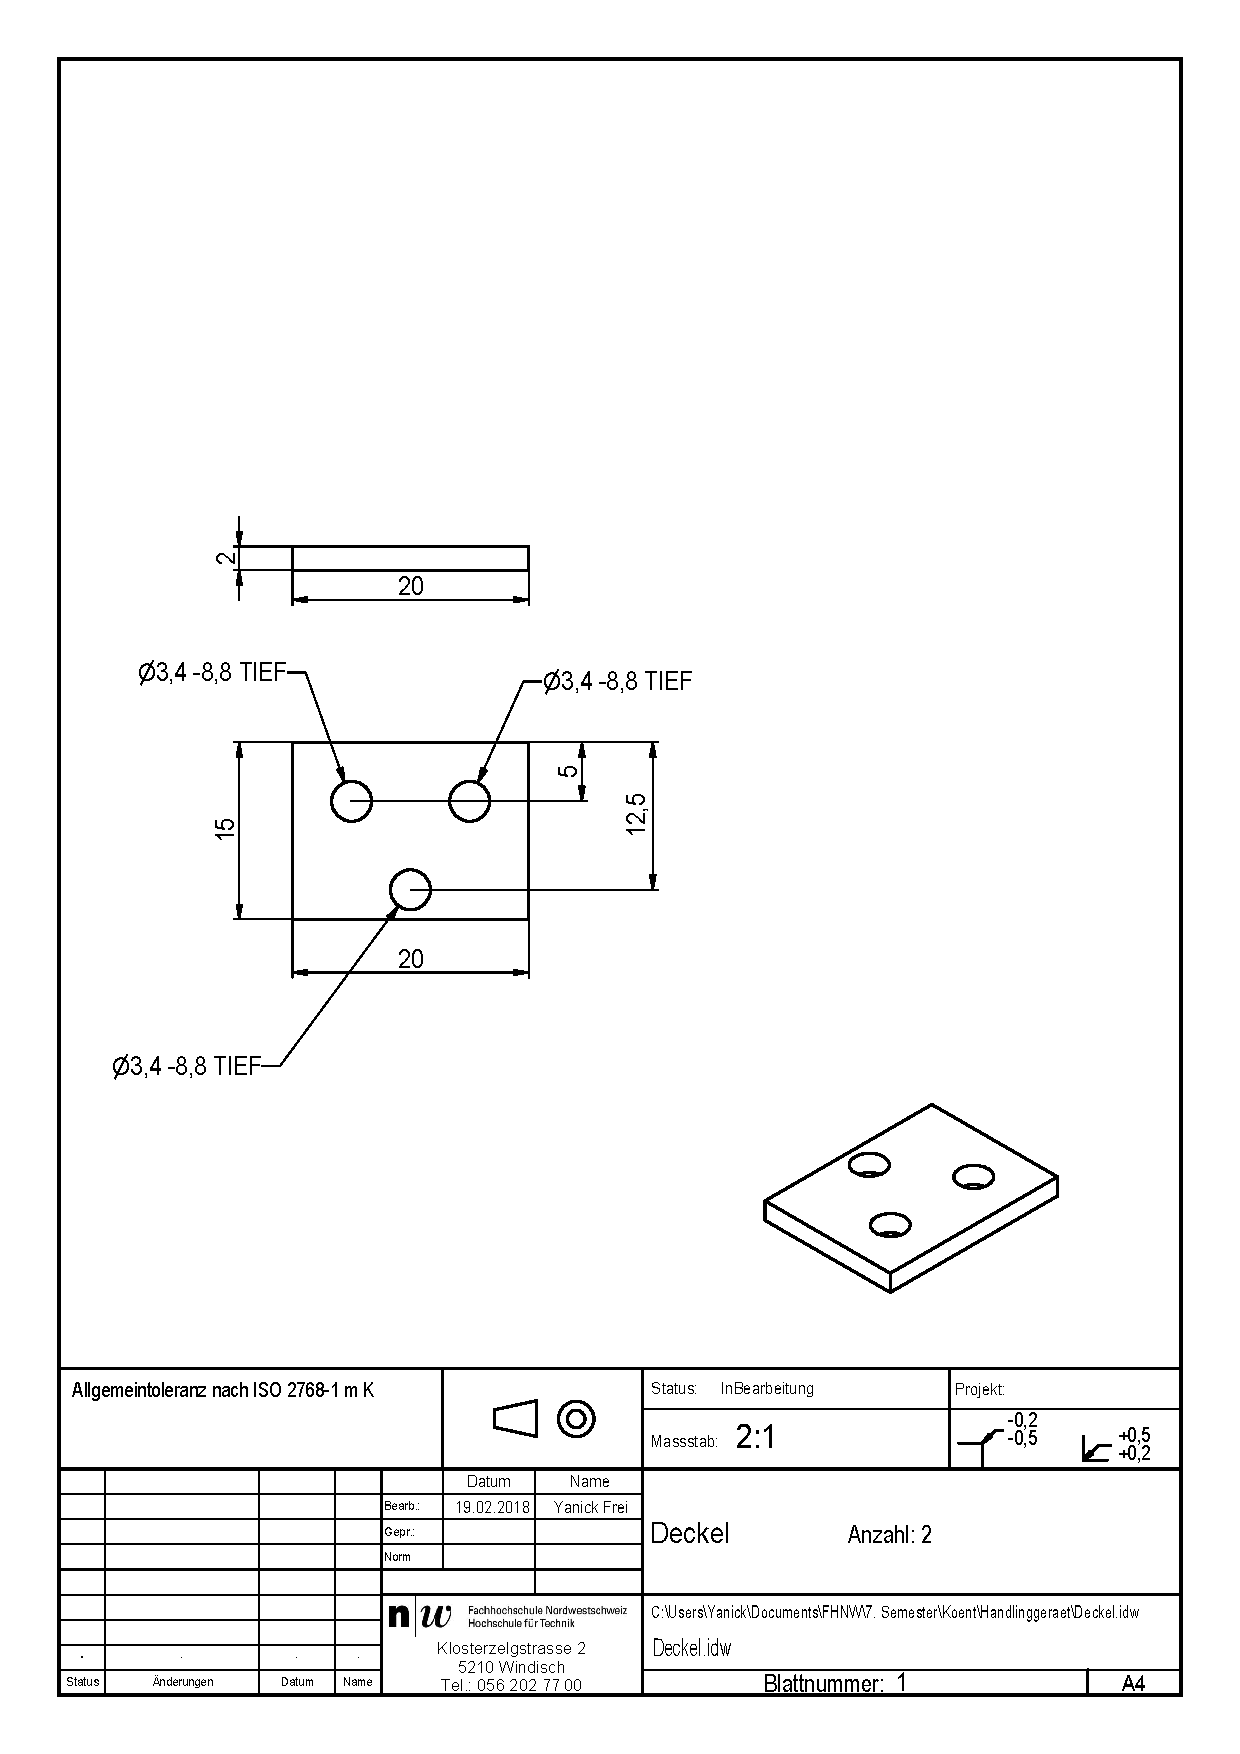
\includepdf{images/Deckel.pdf}

\begin{landscape}
\chapter{Querschnittbestimmung}\label{app:nin}
\begin{minipage}{0.35\textwidth}
		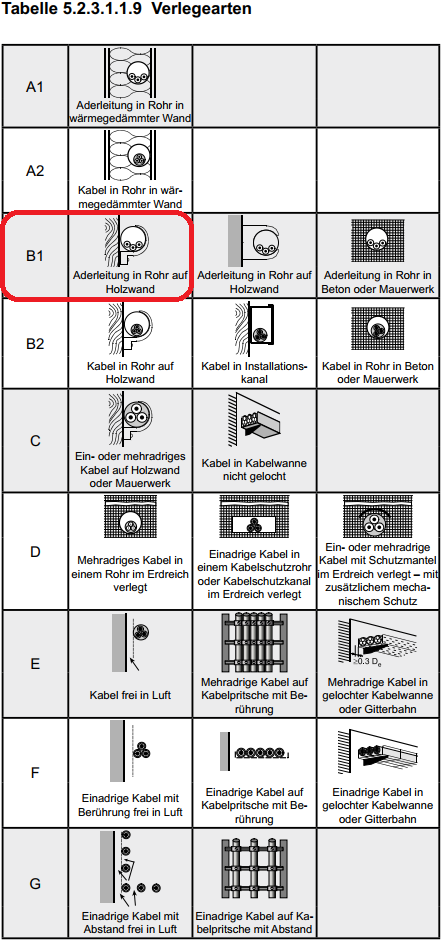
\includegraphics[height=.80\textheight]{images/NIN_Art.png}
	Als Verlegeart wurde \textit{Kabel in Rohr auf Holzwand} gewählt, was der Kategorie \textit{B2} entspricht \cite{NIN}
\end{minipage}
\begin{minipage}{0.1\textwidth}
\hspace{2cm}
\end{minipage}
\begin{minipage}{0.55\textwidth}
		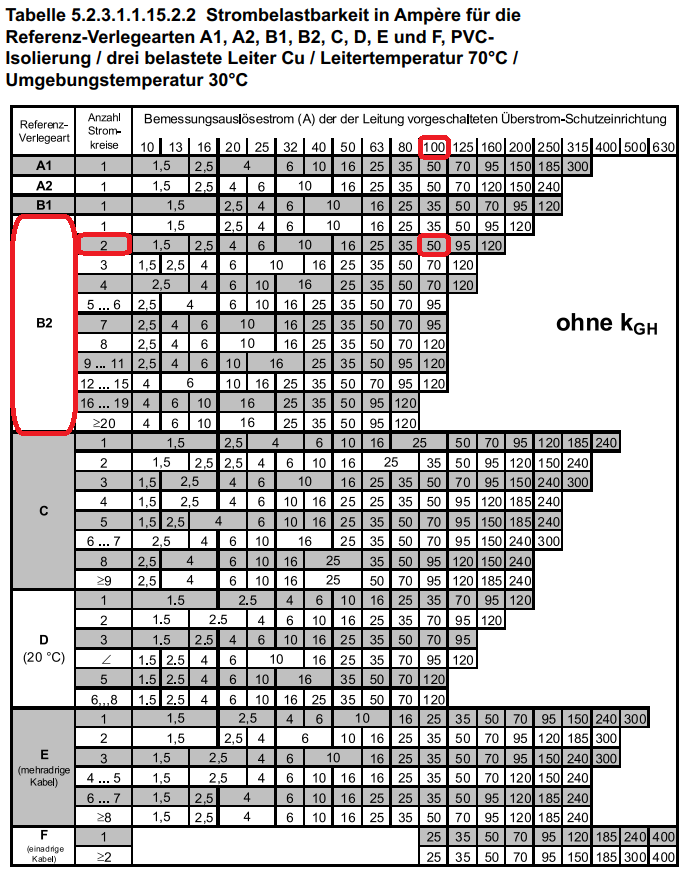
\includegraphics[height=.8\textheight]{images/NIN_Strom.png}
	Für die Verlegeart \textit{B2} mit zwei Stromkreisen und einer $100$ A Sicherung wird ein Querschnitt von $50$ mm$^2$ empfohlen \cite{NIN}
\end{minipage}
\end{landscape}